% https://www.sharelatex.com/blog/2013/08/27/tikz-series-pt1.html

\documentclass[beamer]{standalone}
\usepackage{lmodern}
\usepackage{tikz}
\usetikzlibrary{calc}
\def \stencilradius{6}
\begin{document}
\begin{frame}
  \frametitle{Stencil Codes - Dependency Propagation}
  \begin{figure}
    \centering
    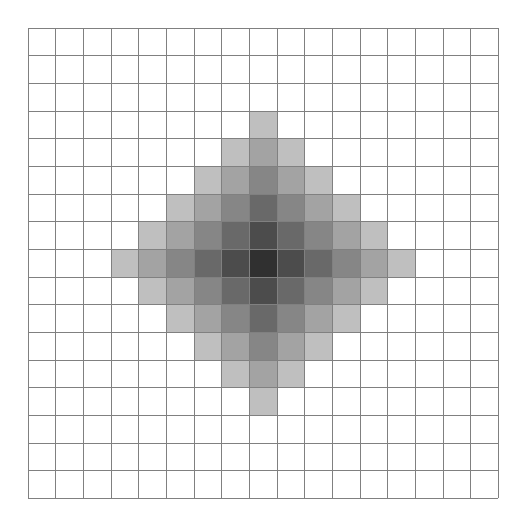
\begin{tikzpicture}[x=1em,y=1em]
      \def \maxrow {16}
      \def \maxcol {16}
      \def \originx{8}
      \def \originy{8}
      
      \foreach \sr in {1,...,\stencilradius}
      {
        \foreach \layer in {\sr,...,1}
        {
          \foreach \r in {0,...,\maxrow}
          {
            \foreach \c in {0,...,\maxcol}
            {
              \pgfmathparse{int(abs(\r - \originx) + abs(\c - \originy))}
              \ifnum \pgfmathresult < \layer
              \pgfmathparse{(\sr - \layer) * 15}
                \fill<\sr>[black!\pgfmathresult!lightgray] (\r,\c) rectangle (\r+1,\c+1);
              \fi
            }
          }
        }
      }
      \draw[step=1, gray, very thin] (0,0) grid (\maxrow+1, \maxcol+1);
    \end{tikzpicture}
  \end{figure}
\end{frame}
\end{document}
